\documentclass[]{article}
\usepackage{amsmath}
\usepackage{amssymb}
\usepackage{verbatim} %con verbatim escribes bloques de texto con letra mono.
\usepackage{graphicx} %para insertar imagenes, cuando meta yo una usa el codigo de ejemplo
\usepackage{listings}
\usepackage{fullpage}
\usepackage{color}
\usepackage{fancyvrb}
\usepackage[spanish]{babel}
\usepackage[utf8]{inputenc} %Para usar acentos directamente en latex
\usepackage{hyperref} %Para que el indice tenga hiperenlaces y si quieres poner los tuyos
\hypersetup{%
	pdfborder = {0 0 0}
}

\definecolor{mygreen}{rgb}{0,0.6,0}
\definecolor{mygray}{rgb}{0.5,0.5,0.5}
\definecolor{mymauve}{rgb}{0.58,0,0.82}

%Para insertar código: crea un recuadro con texto mono y lineas enumeradas. Puedes referenciar un fichero y no copiar y pegar aquí.
\lstset{ %
	backgroundcolor=\color{white},   % chohttp://xdxd.com/ose the background color; you must add \usepackage{color} or \usepackage{xcolor}
	basicstyle=\footnotesize,        % the size of the fonts that are used for the code
	breakatwhitespace=false,         % sets if automatic breaks should only happen at whitespace
	breaklines=true,                 % sets automatic line breaking
	captionpos=b,                    % sets the caption-position to bottom
	commentstyle=\color{mygreen},    % comment style
	frame=single,                    % adds a frame around the code
	keepspaces=true,                 % keeps spaces in text, useful for keeping indentation of code (possibly needs columns=flexible)
	numbers=left,                    % where to put the line-numbers; possible values are (none, left, right)
	numbersep=5pt,                   % how far the line-numbers are from the code
	numberstyle=\tiny\color{mygray}, % the style that is used for the line-numbers
	rulecolor=\color{black},         % if not set, the frame-color may be changed on line-breaks within not-black text (e.g. comments (green here))
	showspaces=false,                % show spaces everywhere adding particular underscores; it overrides 'showstringspaces'
	showstringspaces=false,          % underline spaces within strings only
	showtabs=false,                  % show tabs within strings adding particular underscores
	stepnumber=1,                    % the step between two line-numbers. If it's 1, each line will be numbered
	stringstyle=\color{mymauve},     % string literal style
	tabsize=4,
	inputencoding=utf8,
	title=\lstname                   % show the filename of files included with \lstinputlisting; also try caption instead of title
}



\title{Seguridad}
\author{José Luis Cánovas Sánchez - 48636907A\\Ezequiel Santamaría Navarro - 20096517Z}

\begin{document}

\maketitle

\begin{abstract}
En esta memoria se describe el desarrollo del apartado 2.1 de las prácticas de Seguridad: Despliegue de servicios de gestión de identidad avanzados mediante biometría y tecnologías SAML y OAuth.
\end{abstract}

\tableofcontents


\section{Introducción}

Como grupo 3 de prácticas, desplegaremos las organizaciones 31 y 32.
El trabajo en grupo ha consistido en que ambos hemos desarrollado y configurado todo conjuntamente, lo que se refleja en nuestro repositorio git de GitHub, donde subimos los scripts de instalación con los que automatizamos la práctica, pues preferimos no usar máquinas virtuales, por los problemas de fluidez y tamaño de las máquinas virtuales. Así podemos trabajar con unos pocos megas de scripts y capturas en cualquier ordenador.


%\begin{center}
%	\includegraphics[width=1\linewidth]{images/}
%\end{center}


\section{Autenticación biométrica}

Desarrollamos una aplicación para \textbf{comparación}, \textbf{identificación} y \textbf{verificación} de huellas dactilares.

\hfil

Primero vamos a ver \textbf{cómo funciona} la aplicación desarrollada, y una vez conocemos todas las funcionalidades que ofrece, veremos cómo lo hemos implementado.

\hfil

Cuando abrimos la aplicación nos encontramos con 4 paneles, dos superiores donde se mostrarán las imágenes de las huellas dactilares, dos inferiores, el izquierdo con los botones de las funcionalidades del programa, además del menú superior, y un panel que muestra en texto la descripción de los resultados mostrados.

Los dos primeros botones, \textit{Calcular 1 huella} y \textit{Comparar 2 huellas} no dependen de la base de usuarios del programa.

Al pulsar el primero se abre un explorador de ficheros para abrir la foto de una huella dactilar. El programa entonces muestra la imagen seleccionada a la izquierda y la analizada a la derecha (se indica así en el cuarto panel), y su matriz en el cuadro de texto correspondiente del tercer panel.

El botón de \textit{Comparar 2 huellas} abre dos veces el explorador de ficheros, y muestra las imágenes analizadas, sus matrices y el porcentaje de similitud entre las huellas.


\begin{center}
	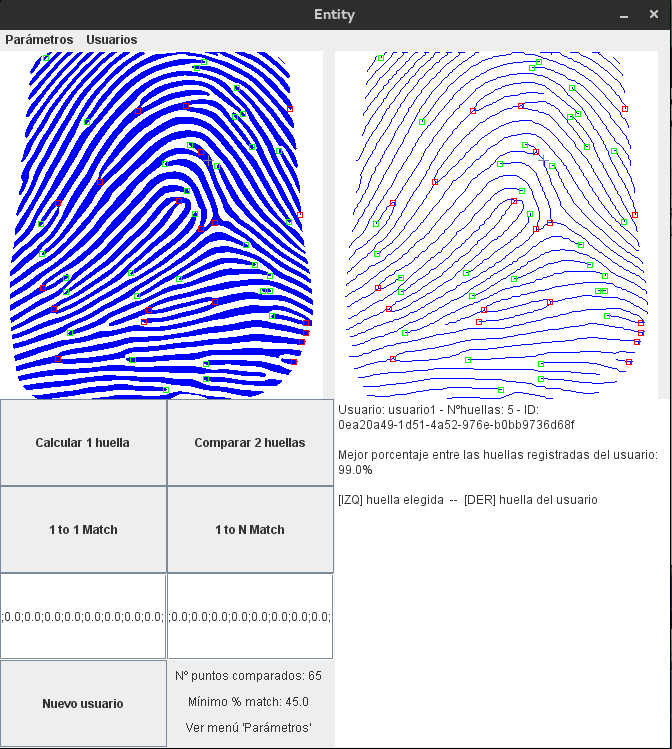
\includegraphics[width=0.55\linewidth]{images/huellas/5.png}

	\textit{Ventana de la aplicación}
\end{center}

Los siguientes botones sí usan la funcionalidad de usuarios del programa. Cuando pulsamos \textit{Nuevo usuario} se abre una ventana nueva donde introducimos su nombre y seleccionamos tantas huellas como queramos para dicho usuario.

\begin{center}
	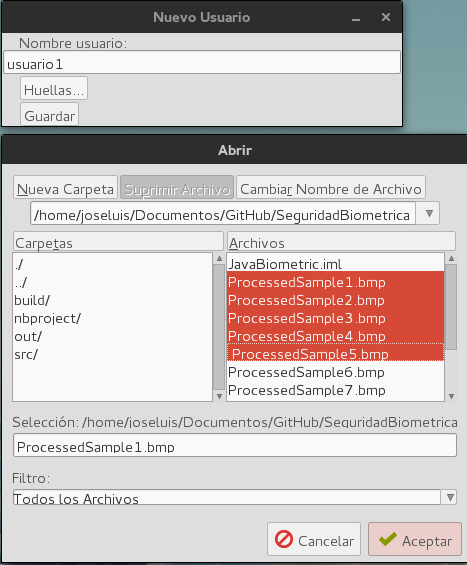
\includegraphics[width=0.45\linewidth]{images/huellas/1.png}

	\textit{Ventana para registrar un nuevo usuario}
\end{center}


Al pulsar en \textit{1 to 1 Match} se realiza una \textbf{verificación} entre un fichero que selecciones en el explorador de ficheros y un usuario de entre los registrados, que se puede elegir de una lista desplegable en una nueva ventana.

\begin{center}
	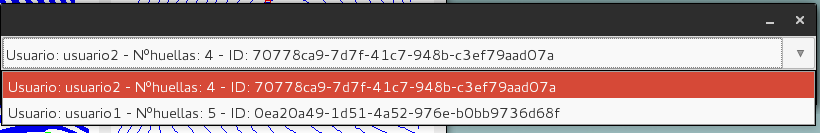
\includegraphics[width=1\linewidth]{images/huellas/3.png}

	\textit{Listado de usuarios para la verificación}
\end{center}

Al pulsar en \textit{1 to N Match} se realiza la comparación de un nuevo fichero que se elija, y todos los usuarios registrados, mostrando la información de los usuarios con las huellas que superan el porcentaje de coincidencia. Se puede probar bajando a un 10\% dicho porcentaje, se mostrará una lista donde cada usuario aparece una sola vez, si alguna de sus huellas supera el porcentaje, y se indica el porcentaje de coincidencia de su huella más coincidente.

\begin{center}
	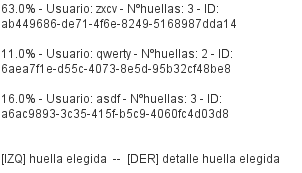
\includegraphics[width=0.5\linewidth]{images/huellas/2.png}

	\textit{Listado de usuarios con huellas que superan el matching}
\end{center}


Por último tenemos las opciones de configuración del menú superior. Tenemos un menú de \textit{Usuarios} con las mismas opciones que ya hemos visto, y un menú de \textit{Parámetros} donde podemos modificar el número de puntos que usará el programa para comparar dos huellas dadas, y el porcentaje mínimo de similitud entre dos huellas para considerar que son de la misma persona.

\begin{center}
	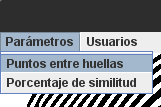
\includegraphics[width=0.25\linewidth]{images/huellas/4.png}

	\textit{Menú Parámetros}
\end{center}

\begin{center}
	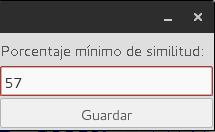
\includegraphics[width=0.25\linewidth]{images/huellas/6.png}

	\textit{Ventana emergente para configurar el porcentaje de similitud}
\end{center}

\begin{center}
	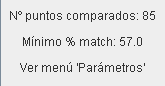
\includegraphics[width=0.25\linewidth]{images/huellas/7.png}

	\textit{Cuadro de texto en el tercer panel con la información de los parámetros actuales}
\end{center}

\hfill

Ahora veamos cómo lo hemos \textbf{implementado}.
\hfill

En la carpeta \textit{src} del proyecto encontramos el fichero \textit{CatalogoUsuarios.java}, donde por un \textit{HashMap} guardamos los usuarios registrados, haciendo uso de la clase \textit{Usuario}, y ofreciendo métodos para la \textbf{identificación}, método \textit{findMatch()}, que devuelve el conjunto de los usuarios que superan el porcentaje de similitud, como se ha descrito en el apartado de la interfaz de usuario.

El fichero \textit{Usuario.java} implementa la representación de cada usuario registrado, mediante un identificador único (asignado automáticamente), un nombre y un conjunto de huellas, representadas por la clase \textit{Huella}. La clase ofrece dos métodos para la \textbf{verificación}, uno que devuelve su huella que mejor coincidencia tiene con otra huella pasada como parámetro, y el otro método devuelve el \textit{double} con el porcentaje de coincidencia.

El fichero \textit{Huella.java} guarda la representación de las huellas dactilares, creándolas a partir del fichero pasado, ofreciendo los métodos para recuperar las imágenes, matriz de la huella calculada (como matriz o string) y el método \textit{coincidencia()} que devuelve el \textbf{porcentaje} de coincidencia entre la huella y otra pasada por parámetro, usando tantos \textbf{puntos} para comparar como configure el usuario.

\hfill

Con estos tres ficheros y la biblioteca \textit{BiometrikSDK} tenemos lo necesario para manipular las huellas y usuarios.

\hfill

En el fichero \textit{ProgramVariables.java} tenemos como parámetros globales los valores que puede ajustar el usuario, número de puntos de comparación entre huellas, y porcentaje mínimo de éxito.

En el fichero \textit{NuevoUsuarioForm.java} se implementa la ventana de registro de un nuevo usuario, y en la acción del botón \textit{Guardar...} se crea el nuevo objeto \textit{Usuario} y se guarda en el catálogo de usuarios.

En el fichero \textit{CEntityForm.java} se implementa el resto de la funcionalidad, la ventana principal del programa, junto a los métodos de los botones, que usan las clases del \textit{CatalogoUsuarios}, \textit{Usuario} y \textit{Huella} para realizar los cálculos y muestran los resultados en el cuarto panel, \textit{panelTexto}.



\clearpage

\section{Escenario de gestión de identidad}

Como grupo 3 desplegaremos las organizaciones 31 y 32. Partimos del escenario inicial de LEGO propuesto en el enunciado, con algunos cambios.
En la siguiente imagen se muestra una imagen con la arquitectura a desarrollar.

\begin{center}
	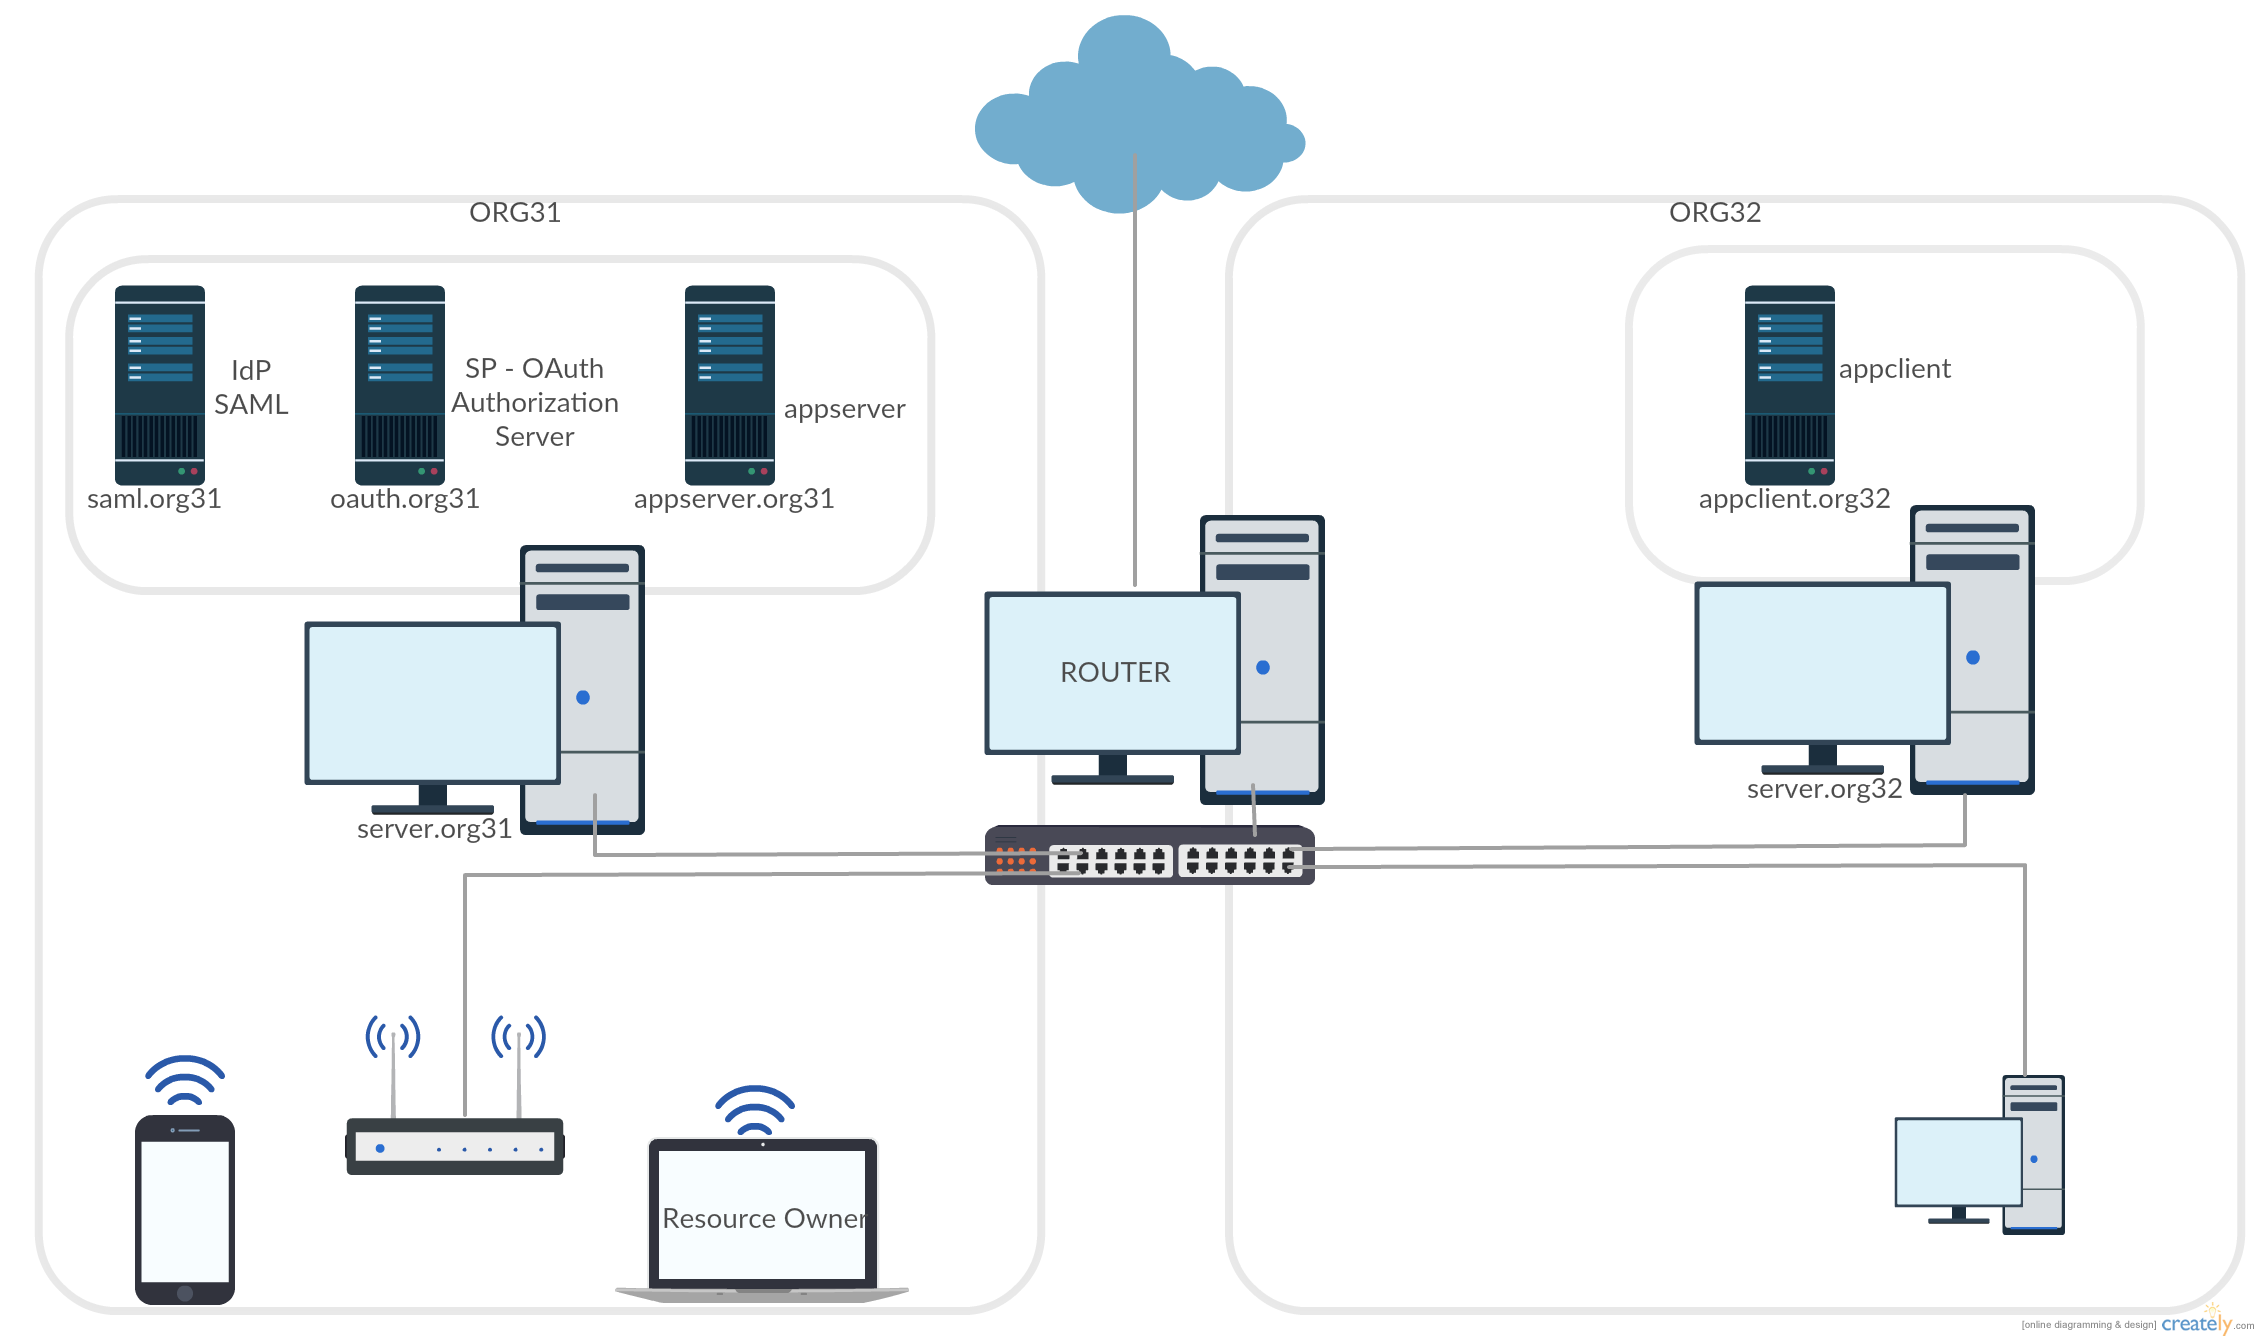
\includegraphics[width=1\linewidth]{images/samloauth/escenario.png}

	\textit{Escenario LEGO de gestión de identidad}
\end{center}

Se nos pide desarrollar un escenario donde el \textit{Resource Owner}, el usuario por medio de su explorador web, se conecta a \textit{appclient.org32},
donde quiere iniciar sesión. Al pinchar en \textit{Login} la web \textit{appclient} le redirige al servidor de \textbf{autorización}, donde pedirá poder acceder
a los datos del usuario para iniciar sesión. Esto se realizará por OAuth con la máquina \textit{oauth.org31}, estando aquí el principal cambio con respecto
a la arquitectura propuesta, que comentaremos por qué más adelante. En este punto \textit{oauth.org31} aún no sabe de qué usuario se trata, por eso necesita que
iniciemos sesión, pero como \textit{oauth.org31} no maneja los usuarios y credenciales, actúa como un \textit{SP} usando SAML con el IdP en la máquina \textit{saml.org31},
la cual sí tiene configurados los usuarios y contraseñas. Una vez nos \textbf{autenticamos} en \textit{saml.org31}, como \textit{Resource Owner} damos permiso en
\textit{oauth.org31} para dar los datos de inicio de sesión a \textit{appclient.org32}.

%TODO: ¿Qué coño hace appserver?
%TODO: mencionar que pensamos que la forma de arreglar eso es poner simplesamlphp en ambas máquinas y modificar los ficheros ya
%configurados para trabajar como idp y sp en la misma máquina a la vez, como un idp y sp en máquinas separadas
%TODO: explicar la resolución de nombres en la bbdd, y mirar los correos que contestaron


\hfill

Hemos cambiado \textit{oauth} de la Organización 32 a la Organización 31 debido a las complicaciones de separar la implementación del proyecto de Phillip Shipley en varias máquinas
en el paso del enlace simbólico. Consideramos que la estructura actual sigue representando una situación de organizaciones realista. Poniendo de ejemplo Google y Doodle,
Doodle sería \textit{appclient} en la Organización 32, y Google sería \textit{oauth} como el servidor de autorización, el que muestra qué cosas compartirás con Doodle, como tu nombre y correo,
también será \textit{saml}, el IdP con el que iniciarás sesión, y puede añadir características extra como el \textit{second factor of authentication}, y también el \textit{appserver} por ejemplo
con la lista de contactos u otro elemento del que hayas dado permisos en la autorización de \textit{oauth}.

Como \textit{saml.org31} y \textit{oauth.org31} pertenecerían ambos a Google, pueden estar en la misma máquina hasta que se resuelva el tecnicismo del enlace simbólico.

\hfill

\subsection{Scripts de instalación}

Para automatizar la configuración del escenario en cualquier máquina, hemos escrito una serie de scripts que no necesitan de interacción manual una
vez se inicia la instalación (excepto algún \textit{Enter} ocasional). Utilizamos la herramienta \textit{make} para facilitar aún más
el despliegue. La organización de los scripts corresponde a una jerarquía de directorios como la siguiente:

\hfil

\begin{BVerbatim}
ROUTER
	Makefile
	network
	test

ORG1
	SERVER
		Makefile
		network
		test
		ESCENARIO
			install.sh
			php-oauth-saml-demo-master
				appserver
				php-oauth
				simplesamlphp
				vagrant

ORG2
	SERVER
		Makefile
		network
		test
		ESCENARIO
			install.sh
			php-oauth-saml-demo-master
				appclient
				vagrant
\end{BVerbatim}

\hfill


Donde ESCENARIO sirve como carpeta contenedora de los scripts específicos de esta práctica, mientras que otros ficheros como \textit{network} nos
permiten configurar LEGO automáticamente, configurando la red, el forwarding, la resolución de DNS o fichero \textit{hosts}, etc.

También usamos otros directorios, como SAML para la práctica 2, u OAUTH para la 3, de donde reutilizamos parte de los scripts para ESCENARIO.


\hfill

En la práctica, para ejecutarlos basta con irse al directorio correspondiente, por ejemplo, para configurar la Organización 31, navegamos a ORG1/SERVER/, y desde ahí
ejecutamos la orden:

\begin{verbatim}
sudo make [network] [escenario] [saml] [test] [...]
\end{verbatim}

Si no ponemos argumentos, por defecto aplicaría la configuración de la red y la del escenario. De querer instalar la práctica 2, deberíamos indicar \textit{saml}, y, por ejemplo, para
probar la configuración, \textit{test}.


\subsection{Configuración de la Organización 31: appserver, php-oauth y simplesamlphp}

\subsection{Configuración de la Organización 32: appclient}



\end{document}
